% ------------------------------------------------------------------------------
% Introduce the topic - What characterizes the topic?
% Introduce the goal - What do you want to achieve with your thesis?
% Make the reader curious - What motivates the reader to read on?
% Describe the relevance - Why is this bachelor thesis scientifically relevant?
%
% The introduction should have the following content:
% - Initial situation & presentation of the topic - You introduce the topic with an exciting 'bait'. You provide initial information on the topic and the object of research and explain the current state of research.
% - Relevance of the topic & motivation - You justify the relevance of your topic (scientifically) and place it in the context of your field. In addition, it is often required that you disclose your personal motivation.
% - Problem description and thematic delimitation - By means of a specific research question (or hypothesis) you present your explicit research interest. If necessary, explain technical terms.
% - Objectives - Your introduction should clearly state what the goal of your paper is and what outcome you hope to achieve upon completion of the bachelor thesis.
% - Method You explain the approach and justify the choice of method.
% - Structure of the Bachelor's thesis - Finally, you give the reader a general overview of your Bachelor's thesis by explaining the structure, showing the red thread and how the research question is answered.
% ------------------------------------------------------------------------------

\opt{never}{\addbibresource{03-tail/bibliography.bib}} % to make citation found in most IDE

\chapter{Introduction}
\label{chap:introduction}

% -- Your text goes here --
For a long time, embedded systems evolved in silos, isolated from each other. However, technology is evolving, and it's time to unite these systems with the world of the \gls{cloud}. Hardware devices have had limitations in terms of resources, although designs have improved these aspects depending on the use case. However, physical limitations remain. The emergence of \hyperref[subsec:cloudcomputing]{cloud computing}, without being for this problem, has offered partial solutions to these challenges.

\hyperref[subsec:cloudcomputing]{Cloud computing} offers a number of advantages, not least the freeing up of hardware resources to optimise the operation of embedded systems. These devices, often limited in their complex processing capabilities, can now benefit from the computing power of the \gls{cloud}. Storage, another constraint, also finds infinite solutions in \hyperref[subsec:cloudcomputing]{cloud computing}, offering virtually unlimited storage capacity. However, the benefits of \hyperref[subsec:cloudcomputing]{cloud computing} are not limited to these aspects. They also include the constant scalability of infrastructures, with independent services that can be easily connected and the possibility of vertical and horizontal scaling.

This development has led to growing interest from engineers looking to interconnect their embedded systems with the \gls{cloud}, a practice now at the heart of the \acrfull{iot}. Faced with increasingly ambitious projects, coupled with the growing integration of artificial intelligence, engineers are looking to \hyperref[subsec:cloudcomputing]{cloud computing} environments to eliminate constraints and facilitate interconnection. To simplify the use of a \gls{cloud_infrastructure}, companies are offering \gls{cloud} platforms providing a multitude of services tailored to different needs (\gls{aws}, Microsoft Azure, etc.). This approach allows engineers to focus more on their business projects rather than spending time maintaining and securing the underlying infrastructure. In this context, the integration of embedded systems with the \gls{cloud} is becoming crucial to meeting the growing demands of the \acrshort{iot}.


% -----------------------------------------------------------------------------
\section{56K.\Gls{cloud}}
\label{subsec:56k.cloud}

% -- Your text goes here --
\nameref{subsec:56k.cloud} is a company established in Sion (Valais) in 2018, specialising in the provision of \gls{cloud}-related services. It offers digital transformation to businesses looking to optimise their processes while reducing their costs. As a consultancy, it is committed to demystifying the \gls{cloud} for customers who may find it difficult to grasp the concepts of the ever-changing digital world. Its collaborative partnerships enhance its skills, enabling it to deliver complete solutions to customers. In order to share its vision of the \gls{cloud} more widely, \nameref{subsec:56k.cloud} also has additional premises in Winterthur (Zurich).
\begin{center}
    \begingroup
    
\includegraphics[width=0.5\columnwidth]{introduction/enterprise_logo.png}
    \captionof{figure}{\nameref{subsec:56k.cloud} company logo \cite{enterprise_56k.cloud}}
    \label{fig:enterprise_logo}
    \endgroup
\end{center}
Digital transformation is a global process aimed at integrating digital technologies into all aspects of a company, from its business model and organisational culture to its processes and operations.

As a consultant, \nameref{subsec:56k.cloud} introduces customers to the \nameref{subsec:cloudnative} approach and explores concepts such as \acrshort{devops} and containerisation.f \acrshort{devops} and containerisation.


% -----------------------------------------------------------------------------
\section{Problem}

% -- Your text goes here --
As part of its core business focused on \gls{cloud} solutions, \nameref{subsec:56k.cloud} is also active in the \acrshort{iot} sector. Recently, the company identified a significant problem relating to collaboration between engineers specialising in embedded systems and those from the \gls{cloud} domain. There is a growing demand for engineers to establish fast and efficient links between embedded devices and \glspl{cloud_infrastructure}. However, there is currently a lack of reference architectures for deploying an infrastructure while directly provisioning a fleet of embedded systems. A reference architecture is a preconceived model for a particular domain. It provides a solid foundation on which other architectures can be built, simplifying the work of software developers in that specific domain.

This problem stems from the time required and the complexity for engineers to establish the connection between hardware and a \gls{cloud_infrastructure}. Because of specialist skills in two distinct areas, a \gls{cloud} professional will need time to understand and implement an operating system capable of connecting to an infrastructure, while an embedded systems expert will need to acquire knowledge of \gls{cloud_infrastructure} by following \nameref{subsec:cloudnative} best practice.
\begin{center}
    \begingroup
    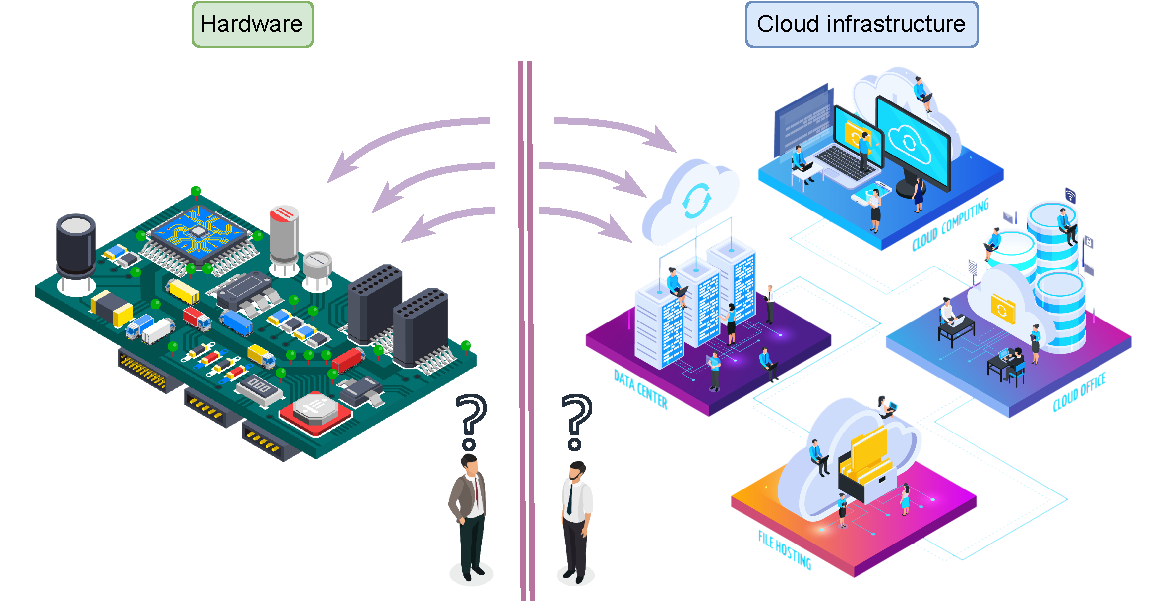
\includegraphics[width=1\columnwidth]{introduction/problem.pdf}
    \captionof{figure}{The problem of linking the hardware to the \gls{cloud_infrastructure} \cite{images_freepik}}
    \label{fig:problem}
    \endgroup
\end{center}
The need to find a solution arose when engineers began to approach electronic board manufacturers to design equipment offering services for linking to a \gls{cloud_infrastructure}. However, these manufacturers, who specialise in hardware, are generally not inclined to devote the time to developing such solutions. The main players affected are hardware engineers, who struggle to meet new customer requirements, and \gls{cloud} engineers, who have to invest time in integrating embedded concepts. This learning phase can quickly become time-consuming.

Although a few solutions are beginning to emerge, most of them remain proprietary. To date, there is no open source reference architecture capable of providing a comprehensive response to the needs of a wide range of products.


% -----------------------------------------------------------------------------
\section{Objectives}

% -- Your text goes here --
The main objective of this project is to design a reference architecture facilitating the deployment of a \gls{cloud_infrastructure} while ensuring the automated provisioning of a fleet of embedded systems. The emphasis is on the ability to provision devices automatically when they are first started up. The infrastructure must contain the essential minimum of services to make the architecture as universal as possible. Since \nameref{subsec:56k.cloud} is a partner of processor manufacturer \gls{arm}, the use of embedded systems equipped with \gls{arm} processors and certified \nameref{sec:arm_systemready} is favoured, in line with the quality standards set by \gls{arm}. The \nameref{sec:arm_systemready} programme guarantees that an operating system and the following software layers can function correctly in their processors.

The infrastructure will be deployed on the \gls{aws} platform, \nameref{subsec:56k.cloud}'s partner \gls{cloud} provider. A fundamental aspect of this project is to promote open source, encouraging the formation of a community around this reference architecture. The aim is to enable engineers specialising in embedded systems and the \gls{cloud} to adopt this architecture easily, while focusing on the development of their end products. \nameref{subsec:cloudnative} best practices are integrated into the development process, while the use of \acrfull{ci} and \acrfull{cd} tools is crucial to ensure a robust architecture. Compatibility must be taken into account to ensure the functionality of the architecture on different embedded systems with \gls{arm} processors and \nameref{sec:arm_systemready} certification.
\begin{center}
    \begingroup
    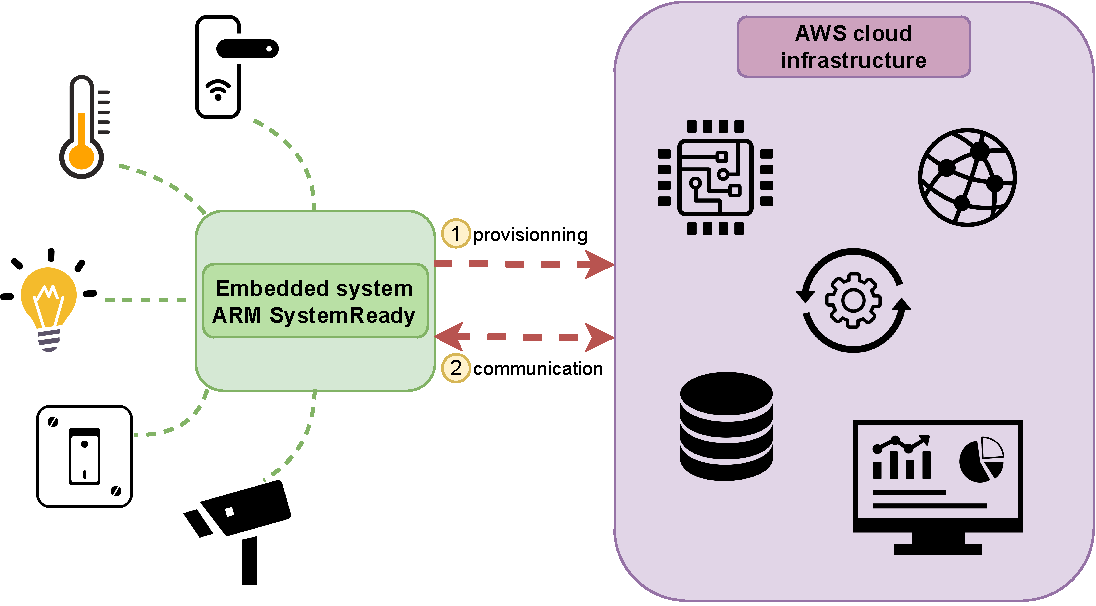
\includegraphics[width=1\columnwidth]{introduction/objective.pdf}
    \captionof{figure}{Overview of objectives}
    \label{fig:objective}
    \endgroup
\end{center}
In parallel with the reference architecture, a small demonstration project is to be based on it. This phase involves deploying a \gls{cloud_infrastructure} on \gls{aws}, with the development of a few applications to be deployed on the embedded systems. The data must pass between these two environments, while offering the possibility of viewing it from a web interface.


% -----------------------------------------------------------------------------
\section{Structure of this report}

% -- Your text goes here --
The \ref{chap:analysis} chapter (\nameref{chap:analysis}) provides important definitions related to the project and examines the state of the art by looking at similar existing solutions.

The \ref{chap:design} chapter (\nameref{chap:design}) provides a comprehensive overview of the reference architecture, encompassing \gls{cloud_infrastructure}, embedded systems integration, the \acrshort{ci}/\acrshort{cd} process and applications.

The \ref{chap:implementation} chapter (\nameref{chap:implementation}) details the implementation of each component of the reference architecture, highlighting the tools used and their functionalities.

The \ref{chap:validation} chapter (\nameref{chap:validation}) analyses the results of the tests carried out on the reference architecture, validating its performance.

The \ref{chap:methodology} chapter (\nameref{chap:methodology}) sets out the project plan, the methodologies adopted and describes the tools used as well as the associated training.

The \ref{chap:conclusions} chapter (\nameref{chap:conclusions}) closes the thesis by presenting the current state of the research, the obstacles encountered and the future directions of the project.